% *********************************************************************
% © 2021–2024 Jeremy Sylvestre
%
% Permission is granted to copy, distribute and/or modify this document
% under the terms of the GNU Free Documentation License, Version 1.3 or
% any later version published by the Free Software Foundation; with no
% Invariant Sections, no Front-Cover Texts, and no Back-Cover Texts. A
% copy of the license is included in the appendix entitled “GNU Free
% Documentation License” that appears in the output document of this
% PreTeXt source code. All trademarks™ are the registered® marks of
% their respective owners.
%
% *********************************************************************

\newcommand*{\tmin}{-2}
\newcommand*{\tmax}{6}
\newcommand*{\ymin}{-1}
\newcommand*{\ymax}{4}

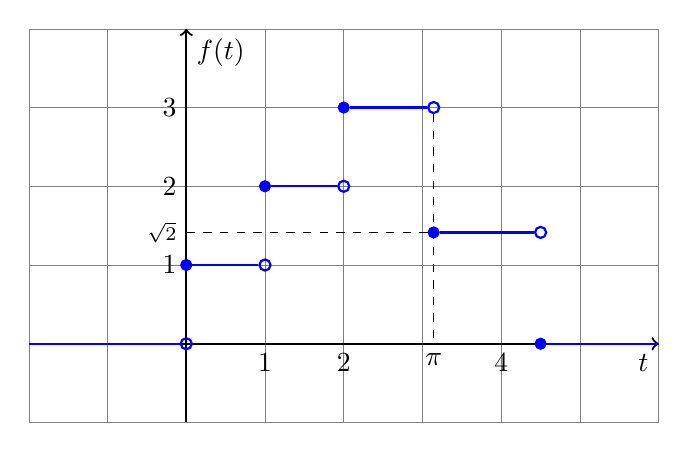
\begin{tikzpicture}
[
	closedpt/.style={circle,draw,fill,inner sep=0pt,minimum size=4pt},
	openpt/.style={circle,draw,inner sep=0pt,minimum size=4pt}
]

	% grid
	\foreach \t in {-2,-1,0,...,6} {
		\draw[very thin,gray] (\t,\ymin) -- (\t,\ymax);
	}
	\foreach \y in {-1,0,1,...,4} {
		\draw[very thin,gray] (\tmin,\y) -- (\tmax,\y);
	}

	% label grid
	\foreach \t in {1,2,4} {
		\node[below] at (\t,0) {$\t$};
	}
	\foreach \y in {1,2,3} {
		\node[left] at (0,\y) {$\y$};
	}

	% axes
	\draw[->,thick] (\tmin,0) -- (\tmax,0) node[below left] {$t$};
	\draw[->,thick] (0,\ymin) -- (0,\ymax) node[below right] {$f(t)$};

	% zero before
	\node[blue,thick,openpt] at (0,0) (stop) {};
	\draw[blue,thick] (\tmin,0) -- (stop);

	% one
	\node[blue,closedpt] at (0,1) (start) {};
	\node[blue,thick,openpt] at (1,1) (stop) {};
	\draw[blue,thick] (start) -- (stop);

	% two
	\node[blue,closedpt] at (1,2) (start) {};
	\node[blue,thick,openpt] at (2,2) (stop) {};
	\draw[blue,thick] (start) -- (stop);

	% three
	\node[blue,closedpt] at (2,3) (start) {};
	\node[blue,thick,openpt] at (3.142,3) (stop) {};
	\draw[blue,thick] (start) -- (stop);
	\draw[dashed,thin] (stop) -- (3.142,0) node[below] {$\pi$};

	% root two
	\node[blue,closedpt] at (3.142,1.414) (start) {};
	\node[blue,thick,openpt] at (4.5,1.414) (stop) {};
	\draw[blue,thick] (start) -- (stop);
	\draw[dashed,thin] (start) -- (0,1.414) node[left] {$\scriptstyle \sqrt{2}$};

	% zero after
	\node[blue,closedpt] at (4.5,0) (start) {};
	\draw[blue,thick] (start) -- (\tmax,0);

\end{tikzpicture}
